\documentclass[12pt,a4paper]{article}
\usepackage[utf8]{inputenc}
\usepackage{ctex} % 支持中文
\usepackage{amsmath, amssymb, amsthm}
\usepackage{graphicx}
\usepackage{listings}
\usepackage{xcolor}
\usepackage{tabularx}
\usepackage{booktabs}
\usepackage{float} % Required for the H float option

\lstset{
    language=Python, % 添加语言支持
    basicstyle=\ttfamily\small,
    numbers=left,
    numberstyle=\tiny,
    keywordstyle=\color{blue},
    commentstyle=\color{gray},
    stringstyle=\color{red},
    breaklines=true,
    frame=single,
    captionpos=b
}

\title{计算流体力学期末大作业}
\author{郑恒2200011086}
\date{\today}

\begin{document}

\maketitle

\section{问题介绍}
针对 Sod 激波管问题,需求解一维欧拉方程:
$$
\frac{\partial U}{\partial t} + \frac{\partial f(U)}{\partial x} = 0
$$
其中:
$$
U = \begin{bmatrix} \rho \\ \rho u \\ E \end{bmatrix}, \quad f(U) = \begin{bmatrix} \rho u \\ \rho u^{2} + p \\ u(E + p) \end{bmatrix}, \quad E = \rho e = \rho \left( C_{v} T + \frac{1}{2} u^{2} \right).
$$
在 $t = 0$ 时刻,初始条件为:
$$
\begin{cases}
x < 0\text{ 处}, & (\rho_{L}, u_{L}, p_{L}) = (1, 0, 1) \\
x \geq 0\text{ 处}, & (\rho_{R}, u_{R}, p_{R}) = (0.125, 0, 0.1)
\end{cases}
$$
要求采用数值方法求解密度、速度、压强分布,并与精确解进行比较。Sod 问题的 Riemann 精确解可查询网络或参考书获得。具体需求如下:
\begin{enumerate}
  \item 计算域与网格由用户设定,并进行相关讨论;
  \item 激波捕捉格式:要求至少完成 TVD、群速度控制(GVC)、WENO 各一种;
  \item 通量处理方法:要求至少完成 FVS(Flux Vector Splitting)和 FDS(Flux Difference Splitting)各一种;
  \item 时间推进格式选用三阶 Runge-Kutta。
\end{enumerate}
\section{算法原理}
\subsection{一维Riemann问题精确解}
根据空气动力学原理,Sod激波管中可能出现三种波类型:
\begin{itemize}
  \item \textbf{激波}:密度、速度、压力均发生突变,满足Rankine-Hugoniot (R-H) 关系式
  \item \textbf{接触间断}:仅密度发生突变,速度与压力不变
  \item \textbf{膨胀波(稀疏波)}:等熵波,内部物理量连续光滑,头尾物理量连续但导数不连续(弱间断),Riemann不变量不变
\end{itemize}

\begin{figure}[H]
    \centering
    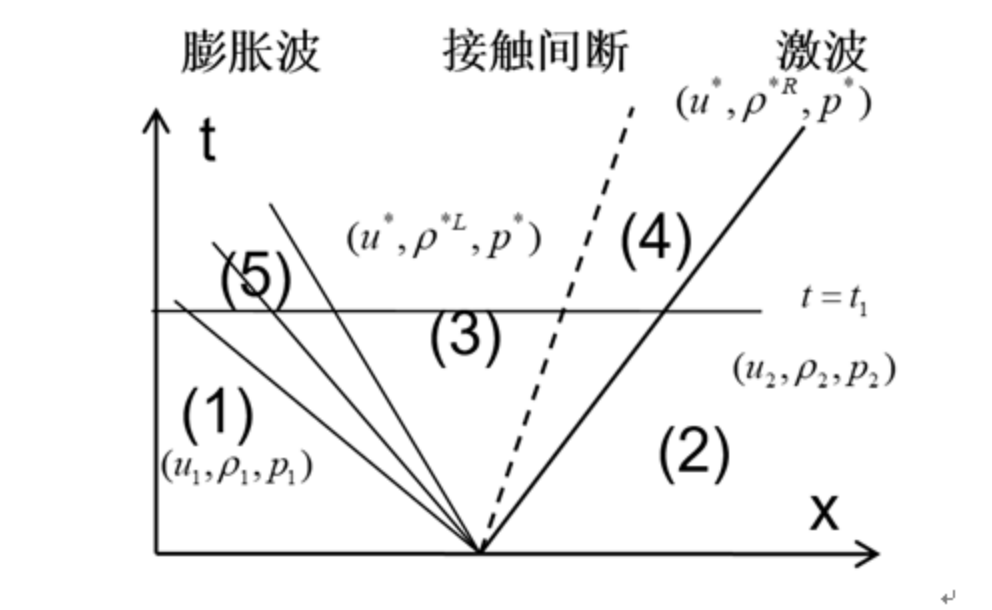
\includegraphics[width=0.7\textwidth]{sod_shock_tube.png}
    \caption{Sod激波管问题示意图}
    \label{fig:sod_shock_tube}
\end{figure}
针对Sod激波管实际工况(初始条件:$(\rho_L, u_L, p_L) = (1, 0, 1)$,$(\rho_R, u_R, p_R) = (0.125, 0, 0.1)$),其流场演化属于\textbf{右激波+左膨胀波}组合。基于质量、动量、能量通量守恒,可建立方程组求解。

\subsubsection{Sod管实际工况:右激波+左膨胀波}
分区列写方程如下:

\textbf{左膨胀波区(1-3区)}:满足等熵关系和Riemann不变量守恒:
\begin{align}
p^{*}/\left(\rho^{*L}\right)^{\gamma} &= p_{1}/\left(\rho_{1}\right)^{\gamma} \label{eq:isentropic} \\
u_{1} + \frac{2c_{1}}{\gamma-1} &= u^{*} + \frac{2c^{L}}{\gamma-1} \label{eq:riemann_inv}
\end{align}
其中 $c_{1} = \sqrt{\gamma p_{1}/\rho_{1}}$ 为左初始区的声速,$c^{L} = \sqrt{\gamma p^{*}/\rho^{*L}}$ 为膨胀波后的声速。

\textbf{右激波区(2-4区)}:满足激波的Rankine-Hugoniot条件:
\begin{equation}
\left\{\begin{array}{l}
\rho_{2}\left(u_{2}-Z_{2}\right)=\rho^{*R}\left(u^{*}-Z_{2}\right) \\
\rho_{2}u_{2}\left(u_{2}-Z_{2}\right)+p_{2}=\rho^{*R}u^{*}\left(u^{*}-Z_{2}\right)+p^{*} \\
E_{2}\left(u_{2}-Z_{2}\right)+u_{2}p_{2}=E^{*R}\left(u^{*}-Z_{2}\right)+p^{*}u^{*}
\end{array}\right. \label{eq:rh_shock}
\end{equation}
其中总能 $E_{k} = p_{k}/(\gamma-1) + \rho_{k}u_{k}^{2}/2$。

激波和膨胀波引起的速度-压力变化可统一表示为:
\begin{align}
\text{左膨胀波:}\ u^{*} &= u_{1} - f\left(p^{*}, p_{1},\rho_{1}\right) \label{eq:left_wave} \\
\text{右激波:}\ u^{*} &= u_{2} + f\left(p^{*}, p_{2},\rho_{2}\right) \label{eq:right_wave}
\end{align}
其中$f$函数定义为分段形式:
\begin{equation}
f\left(p^{*}, p_{i}, \rho_{i}\right)=\left\{\begin{array}{ll}
\dfrac{p^{*}-p_{i}}{\rho_{i} c_{i}\left[\dfrac{\gamma+1}{2\gamma}\left(\dfrac{p^{*}}{p_{i}}\right)+\dfrac{\gamma-1}{2\gamma}\right]^{1/2}}, & p^{*}>p_{i} \quad \text{(激波情况)} \\
\dfrac{2c_{i}}{\gamma-1}\left[\left(\dfrac{p^{*}}{p_{i}}\right)^{\frac{\gamma-1}{2\gamma}}-1\right], & p^{*}<p_{i} \quad \text{(膨胀波情况)}
\end{array}\right. \label{eq:f_function}
\end{equation}

联立方程(\ref{eq:left_wave})和(\ref{eq:right_wave}),得到关于$p^*$的非线性方程:
\begin{equation}
u_{1} - u_{2} = f\left(p^{*}, p_{1},\rho_{1}\right) + f\left(p^{*}, p_{2},\rho_{2}\right) \label{eq:p_star_eq}
\end{equation}
此方程可通过Newton迭代法求解$p^*$,进而计算$u^*$和各区密度。

\subsubsection{膨胀波内部物理量计算}
膨胀波范围由波头速度$u_{1}-c_{1}$和波尾速度$u^{*}-c^{*L}$确定($c^{*L} = \sqrt{\gamma p^{*}/\rho^{*L}}$)。波区内物理量由自相似解给出:
\begin{align}
c(t,x) &= \frac{\gamma-1}{\gamma+1}\left(u_{1}-\frac{x}{t}\right)+\frac{2}{\gamma+1}c_{1} \label{eq:c_expansion} \\
u(x,t) &= c + \frac{x}{t} \label{eq:u_expansion} \\
p(x,t) &= p_{1}\left(\frac{c}{c_{1}}\right)^{2\gamma/(\gamma-1)} \label{eq:p_expansion} \\
\rho(x,t) &= \gamma p / c^{2} \label{eq:rho_expansion}
\end{align}
此解仅适用于$u_1 - c_1 \leq x/t \leq u^* - c^{*L}$区域。

综上所述,一维 Riemann 问题的精确解的求解思路与方程介绍完毕。本文 Sod 激波管参考精确解程序来自于github开源项目,地址为

https://github.com/sbakkerm/Sod-Shock-Tube/tree/main。
\subsection{时间推进格式}
时间推进采用三阶 Runge-Kutta 方法,整个离散格式为:
\begin{align}
\frac{\partial U}{\partial t} &= -\frac{\partial \mathbf{F}}{\partial x} \\
U^{(1)} &= U^{n} - \Delta t \cdot \frac{\partial \mathbf{F}}{\partial x}(U^{n}) \\
U^{(2)} &= U^{n} - \frac{\Delta t}{2} \cdot \frac{\partial \mathbf{F}}{\partial x}(U^{(1)}) \\
U^{(3)} &= U^{n} - \frac{\Delta t}{2} \cdot \frac{\partial \mathbf{F}}{\partial x}(U^{(2)}) \\
U^{n+1} &= U^{n} - \frac{\Delta t}{6} \left( \frac{\partial \mathbf{F}}{\partial x}(U^{(1)}) + 2\frac{\partial \mathbf{F}}{\partial x}(U^{(2)}) + 2\frac{\partial \mathbf{F}}{\partial x}(U^{(3)}) \right)
\end{align}
其中 $\mathbf{F}$ 是通量函数,$\Delta t$ 是时间步长。

其中守恒向量 $U$ 和通量函数 $\mathbf{F}$ 为:
$$
U = \begin{bmatrix}
\rho \\
\rho u \\
E
\end{bmatrix},
\quad
\mathbf{F} = 
\begin{bmatrix}
\rho u \\
\rho u^{2} + p \\
u(E + p)
\end{bmatrix}
$$



\section{代码实现}

\newpage   
\section{结果分析}

\section{AI工具使用说明表}
\begin{table}[!htbp]
    \centering
    \begin{tabular}{|c|c|c|}
        \hline
        \textbf{AI名称} & \textbf{生成代码功能} & \textbf{使用内容} \\
        \hline
        Copilot & latex格式框架 & figure参数调整、图片插入\\
        \hline
        Deepseek & python绘图调整 & 68-90行图绘制的具体参数调整\\
        \hline
        Deepseek & gitignore文件忽略 & 全由ai添加\\
        \hline
\end{tabular}
\end{table}
\section{commit信息}
commit图如下:


\end{document}